\documentclass{article}
\usepackage{listings}
\usepackage{tikz}
\usetikzlibrary{matrix}
\usepackage{pgfplots}
\usepgfplotslibrary{fillbetween}

\usepackage{mathpazo}
\usepackage{amsmath}
\usepackage{cite}

\newcommand\hlight[1]{\tikz[overlay, remember picture,baseline=-\the\dimexpr\fontdimen22\textfont2\relax]\node[circle,fill=blue!50,rounded corners,fill opacity = 0.2,draw,thick,text opacity =1] {$#1$};} 

\newcommand{\hhlline}[3]{\draw (#1-#2-2.south west) -- (#1-#2-#3.south east);}
\tikzset{elegant/.style={smooth,thick,samples=50,cyan}}
\tikzset{eaxis/.style={->,>=stealth}}

\author{Lin Jiaying}
\title{The Design and Analysis of Computer Algorithms
Chapter 7 Exercise Solution}

\begin{document}
	\maketitle
	\section{Question 7.1}
	\paragraph{Solution:}
	We use backward approach(forward reasoning) to solve this finding the shortest route problem.\\
	\begin{align*}
	d(S, A) &= 4\\
	d(S, B) &= 5\\
	d(S, C) &= 1\\
	d(S, D) &= min\{d(S, A) + d(A, D), d(S, B) + d(B, D)\} \\
		    &= min\{4 + 10, 5 + 6\} \\
		    &= 11\\
	d(S, E) &= min\{d(S, B) + d(B, E), d(S, C) + d(C, E)\} \\
	&= min\{5 + 5, 1 + 11\}\\
	&= 10\\
	d(S, F) &= min\{d(S, A) + d(A, F)\}\\
	&= min\{4 + 9\}\\
	&= 13\\
	d(S, G) &= min\{d(S, C) + d(C, G)\}\\
	&= min\{1 + 2\}\\
	&= 3\\
	d(S, T) &= min\{d(S, D) + d(D, T), d(S, E) + d(E, T), d(S, F) + d(F, T), d(S, G) + d(G, T)\}\\
	&= min\{11 + 4, 10 + 3, 13 + 5, 3 + 3\}\\
	&= 6\\
	\end{align*}
	The dynamic programming approach can be explained as there's one solution as follows:\\
	$S \to C \to G \to T$\\
	The length of this solution, namely:\\
	$d(S, C) + d(C , G) + d(G, T) =  1 + 2 + 3 = 6$
	\section{Question 7.5}
	\paragraph{Solution:}
	Since we have the constraints under the linear programming problem like:\\
	Maximize $x_0 = 8x_1+7x_2$\\
	subject to\\
	\begin{align}
	 2x_1 + x_2 &\leq 8 \\
5x_1 + 2x_2 &\leq 15\\
x_1, x_2 &\in N
	\end{align}

	And the $x_1, x_2$ are non-negative integers.\\
	So we can plot all these two constraints inequalities in rectangular coordinate as follows:\\
	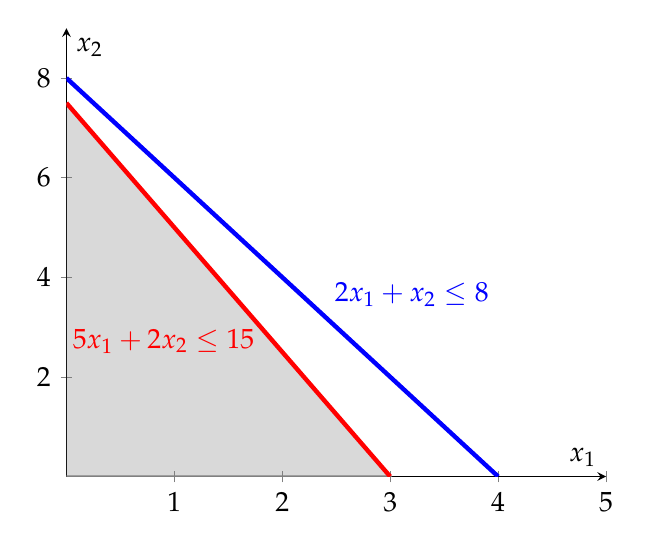
\begin{tikzpicture}
		\begin{axis}[
		axis x line=middle,
		ymax = 9,
		xmax = 5,
		axis y line=middle,
		xlabel=$x_1$,
		ylabel=$x_2$]

		\addplot[thick, color = gray, fill = gray, fill opacity = 0.3]
		coordinates{
		(0,0)
		(3,0)
		(0,7.5)	
	};
		\addplot[elegant, domain = 0:4,ultra thick, blue]{8-2*\x}
		node [pos = 0.8, above = 1cm]{$2x_1 + x_2 \leq 8$};
	\addplot[name path = f, elegant, domain = 0:3,ultra thick, red]{7.5-2.5*\x}
		node[pos = 0.3, below = 1.3cm] {$5x_1 + 2x_2 \leq 15$};
];
		\end{axis}
		
	\end{tikzpicture}
	\\
	We assume the $x_1, x_2$ are not only the integer but also the non-negative real number in the rectangular coordinate since this assumption doesn't affect our relation between the two major constraints.\\
	Under our assumption, we can see that the "red" one constraint is under the "blue" constraint, which means that, exactly, the (2) inequlity decides all our constraint. Also, in algebra way we also can prove this point, since they don't have a solution in the first quadrant. \\
	If we can promise that the (2) equality is satisfied, the (1) will be also satisfied, so our problem can be transformed into this smaller problem:\\
	Maximize $x_0 = 8x_1+7x_2$, subject to:\\
	\begin{align*}
	5x_1 + 2x_2 &\leq 15\\
	x_1, x_2 &\in N\\
	\end{align*}
	\\
	Obviously, it's a complete knapsack problem in a variant way, which has been studied by\cite{dp}, and it was demonstrated that this pattern of linear programming could be considered as the complete knapsack problem.\\
	We will solve this problem as a complete knapsack problem as follows:\\
	\\
	In 0/1 knapsack problem we studied, we have N objects and we can only choose them once, which in this problem means that the constraints we use like:\\
		\begin{align*}
	\sum_{i = 1}^{N} W_{i}x_i &\leq b\\
	x_i &\in\{0,1\}
	\end{align*}
	However, in this complete knapsack problem, we have:\\
		\begin{align*}
\sum_{i = 1}^{N} W_{i}x_i &\leq b\\
x_i &\in\{0,1, 2, ... , \lfloor \frac{b}{a_i} \rfloor \}
\end{align*}
	\\
	,but we can still use the recursive formula like the 0/1 knapsack problem we discussed before to solve this problem, similarly, this complete knapsack problem have a recursive formula as follows:\\
	Let $f_{i}(Q)$ be the value of an optimal solution to objects 1,2,3,... ,i with capacity Q.\\
	$$f_{i}(Q) = max\{f_{i-1}(Q), f_{i - 1}(Q - kW_i) + kP_i\}, 1 \leq kW_i \leq Q$$\\
	The optimal solution is $f_{2}(15)$.\\
	$$
	f_{2}(15) = max \left\{
	\begin{aligned}
	 & max\{f_{1}(15), f_{2 - 1}(15 - 1*5) + 1 * 8 \}, k = 1, i = 1\\
	 & max\{f_{1}(15), f_{2 - 1}(15 - 2*5)  + 2 * 8\}, k = 2, i = 1\\
	 & max\{f_{1}(15), f_{2 - 1}(15 - 3*5) + 3 * 8\}, k = 3, i = 1\\
	 & max\{f_{1}(15), f_{2 - 1}(15 - 1*2) + 1 * 7  \}, k = 1, i = 2\\
	 & max\{f_{1}(15), f_{2 - 1}(15 - 2*2) + 2 * 7 \}, k = 2, i = 2\\
	& max\{f_{1}(15), f_{2 - 1}(15 - 3*2) + 3 * 7\}, k = 3, i = 2\\
	 & max\{f_{1}(15), f_{2 - 1}(15 - 4*2)+ 4 * 7 \}, k = 4, i = 2\\
	 & max\{f_{1}(15), f_{2 - 1}(15 - 5*2)+ 5 * 7 \}, k = 5, i = 2\\
	 & max\{f_{1}(15), f_{2 - 1}(15 - 6*2)+ 6 * 7 \}, k = 6, i = 2\\
	 & max\{f_{1}(15), f_{2 - 1}(15 - 7*2)+ 7 * 7 \}, k = 7, i = 2\\
	\end{aligned}
	\right\}
	$$
	\begin{align*}
f_{1}(15) &= \lfloor \frac{15}{5} \rfloor * 8 = 3 * 8\\
&= 24\\
f_{1}(13) &= \lfloor \frac{13}{5} \rfloor * 8 = 2 * 8\\
&= 16\\
f_{1}(11) &= \lfloor \frac{11}{5} \rfloor * 8 = 2 * 8\\
&= 16\\
f_{1}(10) &= \lfloor \frac{10}{5} \rfloor * 8 = 2 * 8\\
&= 16\\
f_{1}(9) &= \lfloor \frac{9}{5} \rfloor * 8 = 1 * 8\\
&= 8\\
f_{1}(7) &= \lfloor \frac{7}{5} \rfloor * 8 = 1 * 8\\
&= 8\\
f_{1}(5) &= \lfloor \frac{5}{5} \rfloor * 8 = 1 * 8\\
&= 8\\
f_{1}(3) &= \lfloor \frac{3}{5} \rfloor * 8 = 0 * 8\\
&= 0\\
f_{1}(1) &= \lfloor \frac{3}{5} \rfloor * 8 = 0 * 8\\
&= 0\\
f_{1}(0) &= \lfloor \frac{0}{5} \rfloor * 8 = 0 * 8\\
&= 0\\
\end{align*}
$$ f_{2}(15) = max \left\{
\begin{aligned}
 & max\{24, 16 + 8 \}, k = 1, i = 1\\
 & max\{24, 8 + 16\}, k = 2, i = 1\\
& max\{24, 0 + 24\}, k = 3, i = 1\\
& max\{24, 16 + 7  \}, k = 1, i = 2\\
 & max\{24, 16 + 14 \}, k = 2, i = 2\\
& max\{24, 8 + 21\}, k = 3, i = 2\\
 & max\{24, 8 + 28 \}, k = 4, i = 2\\
 & max\{24, 8+ 35 \}, k = 5, i = 2\\
 & max\{24, 0 + 42\}, k = 6, i = 2\\
 & max\{24, 0 + 49\}, k = 7, i = 2\\
\end{aligned}
\right\}
$$
$$
f_{2}(15) = 49
$$
Finally, we can get that the optimal solution is $x_1 = 0, x_2 = 7$.\\
$\sum_{1\leq i \leq n} W_{i}x_i	= 7 * 2 = 14 \leq 15$\\
$\sum P_{i}x_i = f_{2}(15) = 49$

\section{Question 7.6}
In LCS problem, we have studied that:
$$
L_{i,j} = \left\{
\begin{aligned}
&0  &\text{i = 0 or j = 0}\\
&L_{i-1,j-1} + 1  &\text{if $a_i = b_j $}\\
&max\{L_{i-1,j}, L_{i, j-1}\}  &\text{if $a_i \neq b_j$}\\
\end{aligned}
\right.\
$$
\\
Let $L_{i,j}$ denote the length of the longest common sequence of $a_1, a_2, ..., a_i$ from A and $b_1, b_2, ... , b_j$ from B.\\
We can draw the LCS table by our recursive relation above.\\
\[
\begin{bmatrix}

	L_{1,1} &	L_{1,2} & L_{1,3} & ... & L_{1,8} \\
	L_{2,1} &	L_{2,2} & 		&	& ...\\
	L_{3,1} &  			& 	\ddots	&  & ...\\
		... &  			& 		&\ddots &  ...\\
	L_{5,1} & ...		& ...	 & .... & L_{5,8}\\
\end{bmatrix}
\]
\\
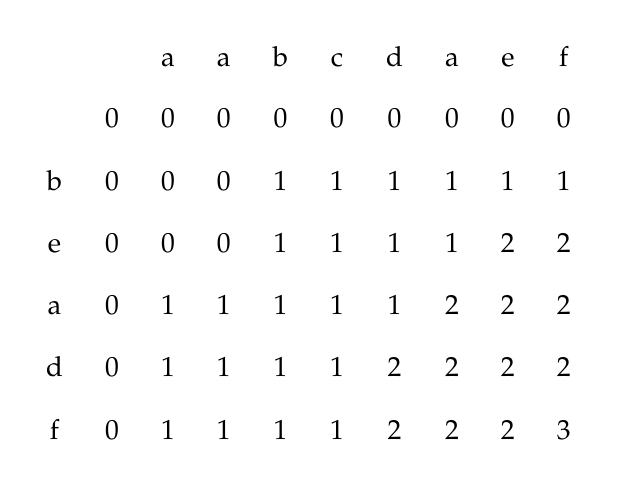
\begin{tikzpicture}[>=stealth]
\matrix (A) [matrix of nodes, row sep = 3mm, column sep = 3mm, nodes in empty cells]
{
  	& 	& a & a & b & c & d & a & e & f  \\
	& 0	& 0 & 0 & 0 & 0 & 0 & 0 & 0 & 0  \\
b	& 0 & 0 & 0 & 1 & 1 & 1 & 1	& 1 & 1  \\
e	& 0 & 0 & 0 & 1 & 1 & 1 & 1 & 2 & 2  \\
a	& 0 & 1 & 1 & 1 & 1 & 1 & 2 & 2 & 2  \\
d	& 0 & 1 & 1 & 1 & 1 & 2 & 2 & 2 & 2  \\
f	& 0 & 1 & 1 & 1 & 1 & 2 & 2 & 2 & 3  \\
};
\end{tikzpicture}
\\
And we can trace back the table to find the LCS for $S_1, S_2$.\\
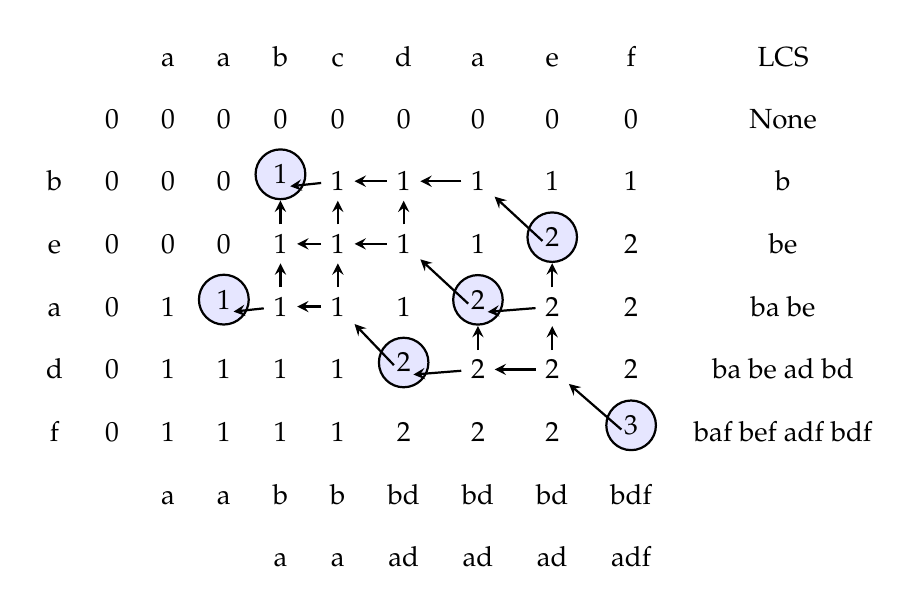
\begin{tikzpicture}[>=stealth]
\matrix (A) [matrix of nodes, row sep = 3mm, column sep = 3mm, nodes in empty cells]
{
		& 	& a & a & b 		 & c & d & a & e & f  	   	 & 	LCS	\\
		& 0	& 0 & 0 & 0 		 & 0 & 0  & 0 & 0 & 0 		 &	None	\\
	b	& 0 & 0 & 0 & \hlight{1} & 1 & 1 & 1	& 1 & 1  	 &	b	\\
	e	& 0 & 0 & 0 & 1 & 1 & 1 & 1 & \hlight{2} & 2       &  be \\
	a	& 0 & 1 & \hlight{1} & 1 & 1 & 1 & \hlight{2} & 2 & 2 &	ba be\\
	d	& 0 & 1 & 1 & 1 & 1 & \hlight{2} & 2 & 2 & 2 		& ba be ad bd	\\
	f	& 0 & 1 & 1 & 1 & 1 & 2 & 2 & 2 & \hlight{3} 		& baf bef adf bdf	\\
		&	& a	& a & b & b  & bd  & bd  & bd  &       bdf            &\\
		&	&	&   & a & a  & ad  & ad  & ad  &       adf            &\\
};

\draw[circle](A-7-10);

\begin{scope}[thick,black,->,auto]
%\draw (A-2-2)--(A-2-3);
\draw (A-7-10)--(A-6-9);
\draw (A-6-9)--(A-6-8);
\draw (A-6-9)--(A-5-9);

\draw (A-6-8)--(A-6-7);
\draw (A-6-7)--(A-5-6);

\draw (A-5-6)--(A-5-5);
\draw (A-5-6)--(A-4-6);

\draw (A-5-5)--(A-5-4);
\draw (A-5-5)--(A-4-5);

%\draw (A-5-4)--(A-4-3);
%\draw (A-5-4)--(A-5-3);

\draw (A-6-8)--(A-5-8);
\draw (A-5-8)--(A-4-7);
\draw (A-4-7)--(A-4-6);
\draw (A-4-7)--(A-3-7);

\draw (A-4-6)--(A-4-5);
\draw (A-4-6)--(A-3-6);

\draw (A-4-5)--(A-3-5);


\draw (A-5-9)--(A-4-9);
\draw (A-5-9)--(A-5-8);

\draw (A-4-9)--(A-3-8);
\draw (A-3-8)--(A-3-7);
\draw (A-3-7)--(A-3-6);
\draw (A-3-6)--(A-3-5);

%\draw (A-5-4)--(A-4-3);
%\draw (A-3-5)--(A-2-4);
\end{scope}

\end{tikzpicture}
\\
So the longest common subsequence of $S_1$ and $S_2$ is bef, baf, adf and bdf.\\

\begin{thebibliography}{0}
		\bibitem[1]{dp}
Shapiro J F. Dynamic Programming Algorithms for the Integer Programming Problem-I: The Integer Programming Problem Viewed as a Knapsack Type Problem[J]. Operations Research, 1968, 16(1):103-121.
	\end{thebibliography}	
\end{document}
\end{document}